\capitulo{3}{Conceptos teóricos}

\section{ETL}
El término ETL (\textit{Extract, Transform, Load}) se refiere al proceso de obtención de datos desde una o varias fuentes, su transformación y carga final en un lugar centralizado para su posterior uso.

\section{Aprendizaje no supervisado}
Dentro de la disciplina de aprendizaje automático, los algoritmos de aprendizaje no supervisado usan datos que no están clasificados o etiquetados previamente, con el objetivo de obtener las relaciones que existan entre los mismos. El tipo de algoritmos más conocidos de este grupo son los de agrupamiento o \textit{clustering}, los cuáles se encargan de encontrar y agrupar las instancias de los datos de entrada en sus grupos correspodientes, atendiendo a criterios como la similitud o las distancias que las separan.

En este trabajo el tipo de algoritmos usados son los de conjuntos de elementos frecuentes. Estos son capaces de encontrar elementos que aparecen de forma conjunta frecuentemente en un gran listado de transacciones. Por ejemplo, estos algoritmos son muy usados para obtener que artículos se compran juntos para hacer sugerencias de compra en tiendas en línea.

\section{Conceptos sobre \textit{League of Legends}}
\label{sec:lol-conceptos}
\subsection{El juego}
\textit{League of Legends} es un videojuego de estrategia multijugador del tipo \textit{MOBA (Multiplayer Online Battle Arena)}, desarrollado por Riot Games y lanzado en 2011, en el que dos equipos de cinco jugadores se enfrentan para destruir la base del equipo enemigo \cite{misc:como-jugar}. Cada jugador controla dentro del juego a un personaje llamado \textbf{campeón}, que pueden seleccionar antes de empezar a jugar, y es único entre los diez jugadores. Al igual que el campeón, los jugadores pueden seleccionar una posición antes de entrar a partida.

Para asegurar la unicidad se lleva a cabo un proceso de \textbf{selección de campeones} (figura~\ref{fig:early-pick}) entre los diez jugadores, ya divididos en dos equipos. Se empieza con una fase de prohibición, en la que cada jugador bloquea un campeón para evitar que se pueda jugar en la partida actual. A continuación se lleva a cabo la fase de selección, en la cual los jugadores van seleccionando su campeón en orden y alternando el equipo. Empieza el primer jugador del primer equipo, seguido van el primer y segundo jugador del segundo equipo, luego segundo y tercero del primer equipo, tercero y cuarto del segundo equipo, cuarto y quinto del primer equipo, y por último, quinto del segundo equipo. La ordenación de los jugadores es aleatoria.

\begin{figure}[h]
	\centering
	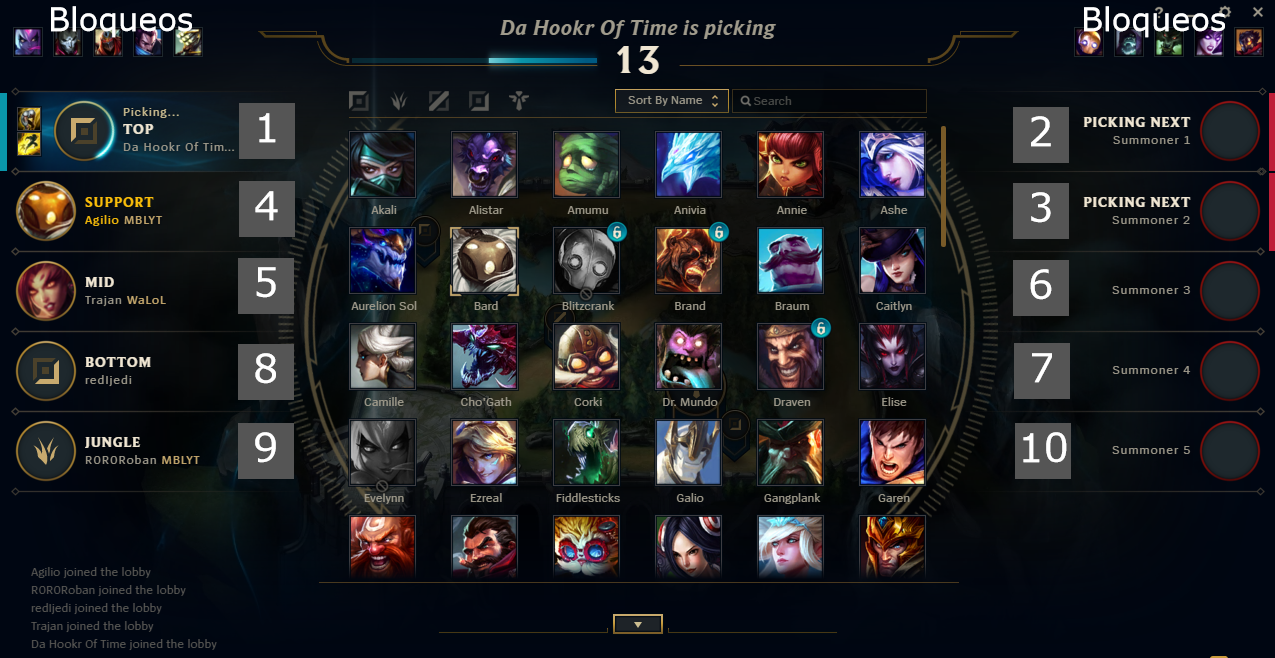
\includegraphics[width=1\linewidth]{img/early-pick}
	\caption{Proceso de selección de campeón}
	\label{fig:early-pick}
\end{figure}

\subsection{Mapa}
Los jugadores se enfrentan en un mapa en forma de cuadrado (figura~\ref{fig:mapa-lol}), con las bases de cada equipo localizadas en zonas opuestas del mapa, una en la esquina inferior izquierda, y la otra en la superior derecha. Conectando cada base se encuentran tres \textbf{líneas} o \textbf{calles}, \textbf{superior} o \textit{\textbf{top}}, \textbf{central} o \textit{\textbf{mid}} e \textbf{inferior} o \textit{\textbf{bot}}. El espacio entre las calles se denomina \textbf{jungla}. Conectando las dos esquinas, que no pertenecen a las bases, se encuentra el \textbf{río} que se encarga de separar el terreno del mapa dominado por cada equipo. De forma general los jugadores se reparten de la siguiente manera, uno en \textit{\textbf{top}}, uno en \textit{\textbf{mid}}, dos en \textit{\textbf{bot}} y el restante en la \textbf{jungla}.

\begin{figure}
	\centering
	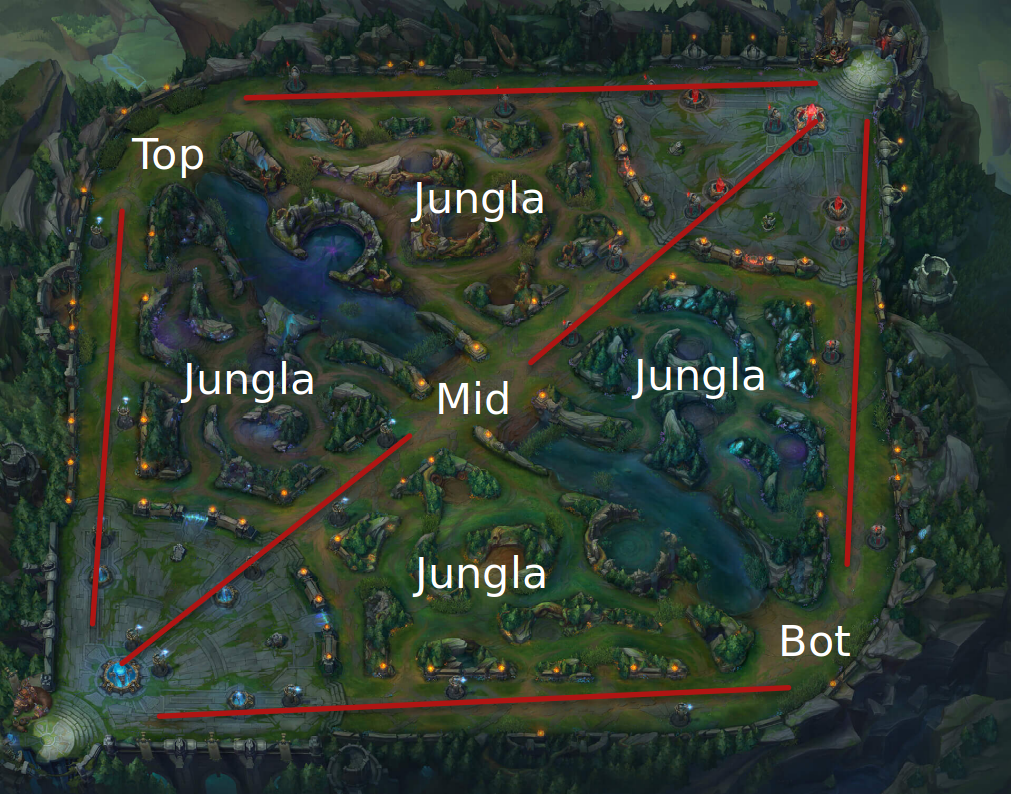
\includegraphics[width=1\linewidth]{img/mapa-lol}
	\caption{Mapa de \textit{League of Legends}.}
	\label{fig:mapa-lol}
\end{figure}

\subsection{Conseguir la victoria}
Para ganar la partida hay que destruir el \textbf{nexo} del equipo enemigo, es la \textbf{estructura} que está más alejada de la base propia. Las \textbf{torres} son otro tipo de estructuras situadas por el mapa, que disparan a los campeones del equipo contrario. Existen tres torres por cada línea y equipo, además de dos adicionales que protegen cada nexo. Las torres se tienen que derribar en el orden que se van encontrando en cada línea, y para destruir el nexo, como mínimo, hay que haber derribado todas las torres de una calle. Aunque un jugador podría moverse por la jungla para llegar a cualquier torre, estas no reciben daño si la anterior sigue en pie.

La forma en la que un equipo consigue ventaja sobre el rival es mediante el \textbf{oro}, este se consigue de varias formas. La principal forma es asesinando a los \textbf{campeones} enemigos. Otras formas de conseguir oro es destruyendo las \textbf{estructuras} enemigas. La última forma de conseguir oro es matando \textbf{monstruos} y \textbf{súbditos}, los primeros se encuentran en la jungla, los segundos recorren las calles en \textbf{oleadas}. Tanto los campeones como los monstruos y súbditos vuelven a aparecer pasado un tiempo concreto, las estructuras, una vez destruidas, no pueden recuperarse.

El oro permite comprar \textbf{objetos}, que mejoran las \textbf{habilidades} del campeón, haciendo que sea más sencillo derrotar a los campeones enemigos, lo que proporciona más oro para más objetos, causando un efecto bola de nieve y la eventual victoria del equipo. Al principio de cada partida, cada jugador empieza con 500 unidades de oro.

Para ver estos conceptos de una forma más visual, Riot Games preparó un vídeo informativo de cara a los mundiales de 2020 para que la gente que no tuviera mucho conocimiento del juego y su funcionamiento pudiera ver y disfrutar la competición. El vídeo se titula \href{https://www.youtube.com/watch?v=ERkt_1TYlkU}{¿Así que queréis ver el Mundial? | Mundial 2020 - League of Legends}\footnote{\url{https://youtu.be/ERkt_1TYlkU}} y se encuentra disponible en YouTube.


\subsection{Campeones}
Los campeones son los diferentes personajes disponibles que un jugador puede seleccionar antes de la partida. Actualmente hay 156 disponibles, añadiéndose a la lista uno nuevo en franjas de tiempo que van desde uno a seis meses. Cada uno tiene un rol asignado que determina su forma de jugar, su función e incluso posición dentro del mapa. Los distintos roles son \textbf{Tirador}, \textbf{Apoyo}, \textbf{Asesino}, \textbf{Luchador}, \textbf{Tanque} y \textbf{Mago}.

Para que un campeón acabe en una categoría u otra hay que prestar atención a varios factores, entre los que se encuentran su \textbf{tipo de ataque} básico, el efecto de sus habilidades y la forma en la que sus estadísticas modifican las \textbf{habilidades}. En las secciones \ref{habilidades} y \ref{estadisticas} se explican en detalles estos conceptos.

\subsection{Habilidades}
\label{habilidades}
Cada campeón tiene un conjunto único de habilidades, una \textbf{pasiva} y cuatro \textbf{activas}, se diferencian en que la pasiva está siempre causando un efecto y las activas causan su efecto cuando decide el jugador. Se pueden definir como las operaciones que un jugador puede realizar para interactuar con el mapa, con otros jugadores, monstruos y súbditos.

Cada habilidad puede tener un efecto o combinar varios, los cuales se aplican sobre uno mismo, un \textbf{aliado} o \textbf{enemigo}. Los efectos más comunes son las \textbf{curaciones}, realizar \textbf{daños} o control de adversario, donde se engloban \textbf{ralentizaciones} o \textbf{inmovilizaciones}. Estos efectos tienen unos valores numéricos que constan de dos partes, un valor base y uno variable que depende de las estadísticas del campeón.

Explicado con un ejemplo, una \textbf{habilidad} de un campeón hace daño a un enemigo con un valor base de 150 puntos de vida y un valor variable que corresponde al 30\% del daño de ataque del campeón. Si en un momento determinado el campeón tiene 300 de daño de ataque, el daño total de la habilidad se calcula como $150 + (0,3 \times 300) = 240$.

En el caso de los daños al rival, existen tres formas en las que se pueden realizar: \textbf{daño físico}, \textbf{mágico} y \textbf{verdadero}. Esto está determinado por la habilidad y rol del campeón.

\subsection{Estadísticas}
\label{estadisticas}
Las estadísticas son diferentes valores numéricos que determinan las capacidades de cada campeón en un área en concreto del juego. \textbf{Estos valores se ven modificados por la compra de objetos (ver sección~\ref{objetos})}. A continuación se describen las estadísticas y que representan.
\begin{description}
	\item[Daño de ataque:] Daño realizado con ataques básicos.
	\item[Probabilidad de crítico:] Probabilidad de que un ataque básico haga el doble de daño.
	\item[Velocidad de ataque:] Cantidad de ataques básicos que se pueden realizar por segundo.
	\item[Poder de habilidad:] Modifica el daño que realizan las habilidades.
	\item[Velocidad de movimiento:] Velocidad a la que un campeón se desplaza por el mapa.
	\item[Armadura:] Cantidad en la que se ve reducido el daño físico que se recibe.
	\item[Resistencia mágica:] Cantidad en la que se ve reducido el daño mágico que se recibe.
	\item[Penetración de armadura:] Cantidad de la armadura del rival ignorada a la hora de realizar daño físico.
	\item[Penetración mágica:] Cantidad de la resistencia mágica del rival ignorada a la hora de realizar daño mágico.
	\item[Vida:] Daño que tiene que recibir un personaje para morir.
	\item[Maná:] Coste de usar habilidades.
	\item[Robo de vida:] Porcentaje de vida recuperado al dañar a un rival.
\end{description}

\subsection{Objetos}
\label{objetos}
Dentro de la base de cada equipo en el mapa está localizada la \textbf{tienda}. Aquí los jugadores pueden comprar objetos con el oro que han ido ganando con el progreso de la partida. \textbf{Su función es modificar las estadísticas del campeón}, para que las habilidades del mismo sean más eficaces contra los rivales. Los objetos que se compran se quedan guardados en el \textbf{inventario} del campeón, el cual está limitado a seis objetos.

En el juego actual existen 222 objetos disponibles, clasificados en cinco categorías:
\begin{description}
	\item[Iniciales:] Objetos más relevantes al inicio de la partida, generalmente mejoran una estadística pero no pueden combinarse para formar un objeto de categoría superior.
	\item[Básicos:] Objetos que mejoran una estadística.
	\item[Épicos:] Objetos formados por la combinación de varios objetos básicos que mejoran varias estadísticas.
	\item[Legendarios:] Objetos formados por la combinación de objetos épicos y/o básicos que mejoran varias estadísticas y proporcionan algún efecto adicional.
	\item[Míticos:] Igual que los anteriores, pero limitado a uno en el inventario.
\end{description}

\subsection{Ligas}
Al igual que otros deportes, \textit{League of Legends} posee un sistema de ligas dentro de las cuales los jugadores que lo deseen pueden clasificarse, en base a la habilidad que demuestren en sus partidas.

En la tabla \ref{tab:ligas} se muestran las diferentes ligas disponibles ordenadas de menor a mayor competencia. También se incluye el porcentaje de jugadores localizados en cada liga \cite{misc:player-distribution} y otros atributos explicados a continuación. El porcentaje no es fijo, los mostrados se refieren al estado de las ligas en agosto de 2021. Esto se debe al movimiento de jugadores entre ligas en base a las partidas que juegan y a los nuevos jugadores que empiezan a jugar.

Desde \textbf{Hierro} a \textbf{Diamante}, cada una cuenta con cuatro divisiones (subcategorías dentro de cada liga), que van desde IV a I. Las tres restantes tienen una única división. Además, tanto \textbf{Gran Maestro} como \textbf{Aspirante} tienen plazas limitadas, 700 y 300 respectivamente.

La localización de cada jugador se basa en un sistema de puntos, ganándolos al salir victorioso y perdiéndolos al ser derrotado, en un rango aproximado de 10-25 puntos por partida. Estos se otorgan en base a una medida numérica oculta a los jugadores llamada \textit{Match Making Rating} (MMR)~\cite{lol_wiki_rank}.

En las ligas con divisiones, cuando el jugador alcanza 100 puntos,  pasa a la siguiente división, o en el caso de estar en la división superior, subiría de liga. Por encima de Diamante no hay límite de puntos, y estando los jugadores ordenados por estos, la clasificación se realiza según el límite de plazas mencionado anteriormente.

\begin{table}[h]
	\begin{tabular}{lrcll}\toprule
		\textbf{Nombre} & \textbf{Porcentaje} & \textbf{Divisiones} & \textbf{Límite usado} & \textbf{Cantidad del límite} \\ \midrule
		Hierro & 1,9\% & IV, III, II, I & Puntos  & 100 por división \\
		Bronce & 19\% & IV, III, II, I & Puntos  & 100 por división \\
		Plata & 37\% & IV, III, II, I & Puntos  & 100 por división \\
		Oro & 28\% & IV, III, II, I & Puntos  & 100 por división \\
		Platino & 11\% & IV, III, II, I & Puntos  & 100 por división \\
		Diamante & 1,4\% & IV, III, II, I & Puntos  & 100 por división \\
		Maestro & 0,11\% & I & Plazas  & Sin límite \\
		Gran Maestro & 0,027\% & I & Plazas  & 700 plazas \\
		Aspirante & 0,011\% & I & Plazas  & 300 plazas \\ \bottomrule
	\end{tabular}
	\caption{Sistema de ligas}
	\label{tab:ligas}
\end{table}


%En aquellos proyectos que necesiten para su comprensión y desarrollo de unos conceptos teóricos de una determinada materia o de un determinado dominio de conocimiento, debe existir un apartado que sintetice dichos conceptos.
%
%Algunos conceptos teóricos de \LaTeX \footnote{Créditos a los proyectos de Álvaro López Cantero: Configurador de Presupuestos y Roberto Izquierdo Amo: PLQuiz}.
%
%\section{Secciones}
%
%Las secciones se incluyen con el comando section.
%
%\subsection{Subsecciones}
%
%Además de secciones tenemos subsecciones.
%
%\subsubsection{Subsubsecciones}
%
%Y subsecciones.
%
%
%\section{Referencias}
%
%Las referencias se incluyen en el texto usando cite \cite{wiki:latex}. Para citar webs, artículos o libros \cite{koza92}.
%
%
%\section{Imágenes}
%
%Se pueden incluir imágenes con los comandos standard de \LaTeX, pero esta plantilla dispone de comandos propios como por ejemplo el siguiente:
%
%\imagen{escudoInfor}{Autómata para una expresión vacía}
%
%
%
%\section{Listas de items}
%
%Existen tres posibilidades:
%
%\begin{itemize}
%	\item primer item.
%	\item segundo item.
%\end{itemize}
%
%\begin{enumerate}
%	\item primer item.
%	\item segundo item.
%\end{enumerate}
%
%\begin{description}
%	\item[Primer item] más información sobre el primer item.
%	\item[Segundo item] más información sobre el segundo item.
%\end{description}
%
%\begin{itemize}
%\item
%\end{itemize}
%
%\section{Tablas}
%
%Igualmente se pueden usar los comandos específicos de \LaTeX o bien usar alguno de los comandos de la plantilla.
%
%\tablaSmall{Herramientas y tecnologías utilizadas en cada parte del proyecto}{l c c c c}{herramientasportipodeuso}
%{ \multicolumn{1}{l}{Herramientas} & App AngularJS & API REST & BD & Memoria \\}{
%HTML5 & X & & &\\
%CSS3 & X & & &\\
%BOOTSTRAP & X & & &\\
%JavaScript & X & & &\\
%AngularJS & X & & &\\
%Bower & X & & &\\
%PHP & & X & &\\
%Karma + Jasmine & X & & &\\
%Slim framework & & X & &\\
%Idiorm & & X & &\\
%Composer & & X & &\\
%JSON & X & X & &\\
%PhpStorm & X & X & &\\
%MySQL & & & X &\\
%PhpMyAdmin & & & X &\\
%Git + BitBucket & X & X & X & X\\
%Mik\TeX{} & & & & X\\
%\TeX{}Maker & & & & X\\
%Astah & & & & X\\
%Balsamiq Mockups & X & & &\\
%VersionOne & X & X & X & X\\
%}
